\documentclass[fleqn,10pt]{wlscirep}
\usepackage{amsmath}
\usepackage{graphicx}
\usepackage{subfigure}
\usepackage{epstopdf}
\usepackage{threeparttable}
\usepackage[rightcaption]{sidecap}
\usepackage{wrapfig}
\usepackage[T1]{fontenc}
\usepackage{underscore}
\usepackage{multirow}
\usepackage[utf8]{inputenc}
\usepackage[T1]{fontenc}
\usepackage[english]{babel}
\usepackage{booktabs}
\setlength{\defaultaddspace}{1ex}
\usepackage{tabularx}
\usepackage{caption} % just for better formatting of table captions

\title{LPI-FKLGCN}
\author[1]{Wen Li}
\author[1,*]{Shulin Wang}
\author[1]{Hu Guo}
\affil[1]{Hunan University, College of Computer Science and Electronic Engineering,Hunan, Changsha, 410082, China}
\affil[*]{corresponding.smartforesting@163.com}

\begin{abstract}
The prediction of lncRNA-protein interaction (LPI) by the computational model can not only help to identify the function of lncRNAs, but also solve the problem of high cost and a long time of biological experiments. In this study, we develop a novel computational model combining machine learning-based fast kernel learning (FKL) and deep learning-based graph convolution network (GCN) encoder to predict potential lncRNA-protein interactions (LPI-FKLGCN). The LPI-FKLGCN model fuses the multi-source lncRNA and protein features into integrated similarity in a fast linear manner and then feeds them into the multi-layer graph convolution network with the known LPIs for encoding. Finally, the two sets of embedding vectors from GCN are decoded to the final LPI score matrix. Through 5-fold cross-validation, LPI-FKLGCN achieves an best AUPR value of 0.52 and an AUC value of 0.96, which is superior to other methods. In the case study, most of the predicted LPIs are confirmed by the newly published biological experiments. This study has shown that the fusion of multi-source similarities and features, combined with multi-layer embedding from graph convolution encoder, can effectively improve the LPI prediction accuracy. It can be seen that LPI-FKLGCN is an efficient and accurate tool for LPI prediction. 
\end{abstract}
\begin{document}

\flushbottom
\maketitle
% * <john.hammersley@gmail.com> 2015-02-09T12:07:31.197Z:
%
%  Click the title above to edit the author information and abstract
%
\thispagestyle{empty}

\section*{Introduction}
Due to the rapid development of high-throughput sequencing technology, tens of thousands of human lncRNAs have been identified in recent years\cite{Chen2013}. It has been found that only about 1\% of the RNA in human transcription encodes proteins, most of which are long non-coding RNAs, whose transcripts are no less than 200 nucleotides, which are not involved in coding protein and have long been considered as transcriptional noise\cite{Engreitz2016}. Long non-coding RNAs (lncRNAs) are RNA molecules that played the role of the regulator in the human body and had an important relationship with cell differentiation, apoptosis, and cancerization\cite{Harrow2012}. Alterations in the primary structure, secondary structure, and expression levels of lncRNAs and their associated RNA-binding proteins underlie a wide range of diseases\cite{Li2014,Wapinski2011}. LncRNAs drive many important cancer phenotypes through interactions with other cellular macromolecules, including DNA, proteins, and RNA \cite{Schmitt2016}. The genomic expression pattern and tissue-specific expression characteristics of lncRNAs in a variety of tissues suggest that lncRNAs have strong prospects as novel biomarkers and therapeutic targets for cancer\cite{Chen2017}. By interacting with related RNA-binding proteins, lncRNAs participate in the regulation of a variety of biological processes and realize their complex and diverse functions\cite{Djebali2012}. Therefore, identifying the interaction between lncRNAs and proteins is of great significance for exploring the cellular mechanisms and molecular functions of lncRNAs and understanding various biological processes related to disease.

Traditional high-throughput biological methods consume a lot of manpower and material resources, and the computational method is a powerful supplement to the former because it is not affected by the expression time, tissue specificity and expression level of non-coding RNA, and can greatly reduce the time and cost. There are a lot of methods proposed for LPI prediction which can roughly be classified into two classes. One class is the original computational model which used only the information contained in the sequences of lncRNAs and proteins to predict whether RNA and protein have interaction. It often integrates some simple statistical methods or machine learning methods to predict. For example, the model of RPISeq encodes the sequences of RNAs and proteins and separately uses support vector machine (SVM) and random forest (RF) classifiers to predict LPIs\cite{Muppirala2011}. Another method that has been proven to work is catRAPID\cite{Bellucci2011}. Lu et al. have introduced a method called lncPro, which encodes RNA and protein sequences into vectors, calculates the score for each RNA-protein pair using matrix multiplication and finally classifies all the RNA-protein pairs according to their scores\cite{Lu2013}. Yi et al. have studied a method based on sequence distributed representation learning, called LPI-Pred, which divides the lncRNA and protein sequences into k-mer segmentation and trains them by RNA2vec and PRO2vec models and predicts the LPIs by the Random Forest\cite{Yi2020a}.

With the development of sequencing technology, LPI information is gradually enriched. The second class LPI prediction method is to combine known LPI information with multi-source lncRNA (protein) data that can be used to extract features and measure similarities. The known interaction information has proved to be very important in interaction prediction. It is hypothesized that if a lncRNA (protein) is similar to one side of the interacting lncRNA-protein pair, it may also interact with the other side of the interacting lncRNA-protein pair. Therefore, similarity calculation is also very important. For example, Zhang et al. have proposed a Sequence-Based Feature Projection Ensemble Learning Method (SFPEL-LPI), which combines multiple similarities and multiple features based on sequence extraction into a feature projection ensemble learning framework to improve the prediction performance\cite{Zhang2018SFPEL-LPI:Interactions}.
Zhao et al. have proposed an algorithm of bipartite network-based projection recommendation for LPI prediction (LPI-BNPRA) which is a semi-supervised method integrating similarities and known interaction knowledge\cite{zhao2018bipartite}. To solve the problem of the lack of negative samples, Zhao et al. also integrate random walk based on network and logical matrix factorization based on semi-supervised machine learning with regularization, which assigns high weights to the nearest neighbours, thereby avoiding noisy\cite{Zhao2018}. Shen et al. have proposed a typical semi-supervised machine learning-based model (LPI-FKLKRR) to identify the potential LPIs, which optimizes the weights of combination by Fast Kernel Learning (FaseKL) and obtain the predicted associations by the Kernel Ridge Regression (KRR)\cite{Shen2019}. Since there are now a limited number of LPIs, some methods have emerged that can be predicted without direct LPIs. Zhou et al. have explored the selection of miRNAs as mediators to establish a heterogeneous network to estimate the potential interactions between lncRNAs and proteins. This model requires no direct prior lncRNA to interact with the protein\cite{Zhou2020PredictingModel}. In recent years, with the development of deep learning methods such as deep neural network and graph neural network, more research efforts are now being put into developing methods that combine machine learning and deep learning to improve predictive performance. For example, Fan et al. have proposed a new computational model LPI-BLS, which integrates a deep learning-based broad learning system with ensemble logistical regression classifiers to predict LPIs \cite{Fan2019LPI-BLS:Classifier}.

Considering the importance of features extracted from sequence information, similarity measurement and known LPI information in previous studies, a new prediction model is proposed in this study, which can not only extract the features of lncRNAs and proteins from multi-source biological data including sequences, lncRNA expression profile and protein Gene Ontology (GO). At the same time, lncRNA-lncRNA and protein-protein similarity are calculated from different perspectives according to different similarity measurement methods. The fast kernel learning method (FKL) based on machine learning is used to fuse these features and similarities respectively to obtain a lncRNA comprehensive similarity and a protein comprehensive similarity. Besides, the comprehensive similarity matrices obtained by the previous fusion of multi-source information and the known lncRNA-protein interaction are sent into the Graph Convolutional Network (GCN) model based on deep learning to extract the two groups of embedding representation vectors, and finally, the LPI probability score matrix is obtained through a decoder. Compared with other baseline methods and the latest methods, the LPI-FKLGCN model performs better. Through case analysis, the proteins and lncRNAs that may be associated with specific lncRNAs can be predicted respectively, and at the same time, the new lncRNAs can be effectively predicted. The workflow of our model LPI-FKLGCN is illustrated in Figure \ref{fig:fig1}.

\begin{figure}[ht]
\centering
\graphicspath{ {./images/} }

\includegraphics[width=\textwidth]{stream.jpg}
%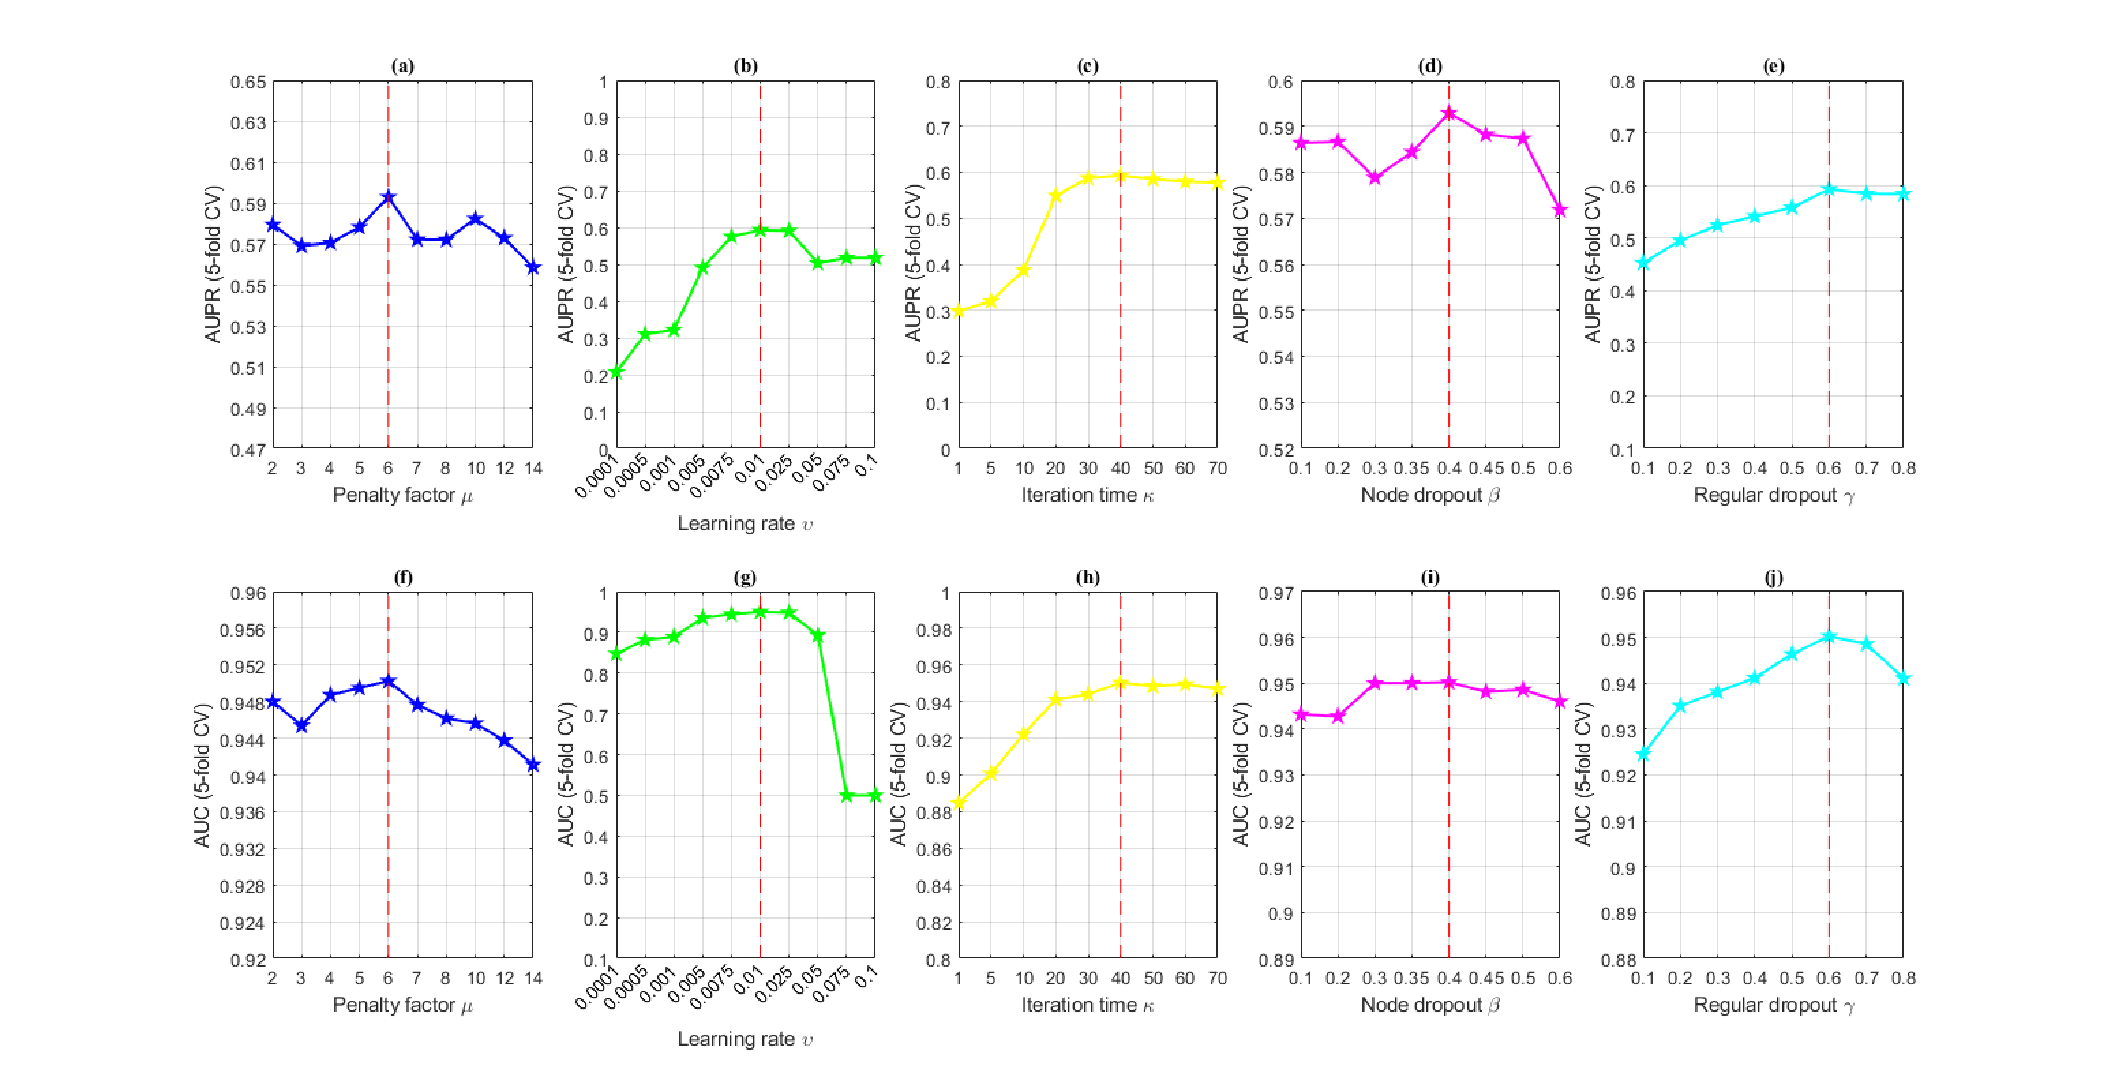
\includegraphics[height=4.5cm,width=7.5cm]{images/fig1_benckmark.pdf}
\caption{The overall framework of LPI-FKLGCN model}
\label{fig:fig1}
\end{figure}

\section*{Results}
\subsection*{2.1 Datasets and experimental environment}
There are two datasets used in this study from previous literature studied by Zhang\cite{Zhang2018} and Zheng\cite{Zheng2017a}, respectively. The Benchmark\_Dataset has 4158 experimentally validated LPIs, including 990 lncRNAs and 27 proteins. To further validate the results on the benchmark dataset, the performance test and comparison test are done on a Novel\_Dataset, which has 4467 experimentally validated LPIs, containing 1050 lncRNAs and 84 proteins. Two datasets are shown in the Table \ref{tab:datasets}. In this section, 5-fold cross-validation (5-fold CV) has been adopted to evaluate the performances of LPI-FKLGCN. All known LPIs are randomly divided into five strictly equal folds. Each fold is taken in turn as a test sample, and the remaining four folds as a training sample. We adopt the Area Under ROC curve (AUC) and Area Under Precision-Recall curve (AUPR)  as primary evaluation metrics. Besides, other metrics such as F1-score (F1), accuracy, recall, specificity and precision are computed in some experiments. All experiments have been done on the computer with 3.59 GHz, 6-core CPU, 32 GB of memory, and 64-bit Windows 10 Professional Operating Systems.
\begin{table}[ht]
\centering
\caption{\label{tab:datasets} The statistics of the datasets used in the experiments (350 words max). Example legend text.}
\begin{threeparttable}[b]
\begin{tabular}{|l|l|l|l|}
\hline
Dataset & \# lncRNA & \# protein & \# interactions \\
\hline
Benchmark_Dataset & 990 & 27 & 4158\\
\hline
Novel_Dataset & 1050 & 84 & 4467 \\
\hline
\end{tabular}
\begin{tablenotes}
     \item "\#" denotes "the number of"
     \end{tablenotes}
     \end{threeparttable}
\end{table}
\subsection*{2.2 Parameter impact analysis}
Cross validation have been performed to analyze the impact of parameters on model performance. There are several parameters in our LPI-FKLGCN model.We tested the penalty factor $\mu$ at the range $\{ 2,3,4,5,6,7,8,10,12,14\} $, iteration time $\kappa$$ \in $$\{ 1,5,10,20,30,40,50,60,70\} $, the learning rate $\upsilon$$ \in $$\{ 0.0001,0.0005,0.001,0.005,0.0075,0.01,0.025,0.05,0.075,0.1\} $, node dropout $\beta$ regular dropout $\gamma$
the total training epochs (*100)= $\kappa$,  the number of layers $h$ in the GCN, 
two dropout rates (node dropout $\beta$ and regular dropout $\gamma$)
the penalty factor $\mu$ in the heterogeneous network.  
By adjusting the parameters empirically,
we set the dimensionality of embeddings k = 64, the number of layers H = 3, 
$\upsilon$ = 0.01, iteration time $\kappa$ = 40, $\beta$ = 0.4, $\gamma$ = 0.6 and $\mu$ = 6 for LPI-FKLGCN in the following experiments

As shown in Figure \ref{fig:fig2-1},When the values of parameters vary in a wide range, the AUC and AUPR values of the model fluctuate little.Thus, the FKLGCN schema is robust.

LAGCN makes use of the drug–disease heterogeneous network to build the prediction model. The drug–disease heterogeneous network consists of known drug–disease associations, drug–drug similarities and disease–disease similarities. Since we consider five types of drug features and two similarity measures, we can train LAGCN on different heterogeneous networks based on different drug–drug similarities, and then discuss how these drug–drug similarities influence the performances of LAGCN.
LAGCN models based on heterogeneous networks with different drug–drug similarities are evaluated by 5-CV on the main dataset, and the corresponding results are displayed in Table 2.
Jaccard index leads to slightly better results than Cosine similarity measure, and similarities based on different features produce similar performances. These results indicate that LAGCN is robust, regardless of similarity measures and drug features. Drug target-based similarities (by both Jaccard index and Cosine similarity) leads to the highest AUPR score. Moreover, we only use the drug–disease associations to construct the network, and then build a reduced version of LAGCN based on this network, named as LAGCN-NH. According to Table 2, LAGCN-NH produces lower AUPR score and AUC score than all LAGCN models, which demonstrates that the drug–drug similarities and disease–disease similarities in the heterogeneous network contain useful information and lead to the improved performances of LAGCN.

We also integrate different drug feature-based similarities using two simple strategies, and build LAGCN models. The average similarity strategy calculates the average of drug–drug similarities based on different features to obtain the integrated similarities. The concatenated feature-based similarity strategy firstly concatenate different drug feature vectors and then calculate drug–drug similarities based on the concatenated feature vectors. The results in Table 2 show that integrating different drug feature-based similarities do not necessarily lead to improved performances. The possible reason is that the known drug–disease associations make the major contribution to the prediction, and drug features bring supplementary information but have redundant information between them. Based on the above discussion, we adopt the target-based drug–drug similarities calculated by the Jaccard index, MeSHbased disease–disease similarities and drug–disease associations to construct the heterogeneous network and then build the LAGCN models in the following study

\begin{figure}[ht]
\centering
\graphicspath{ {./images/} }
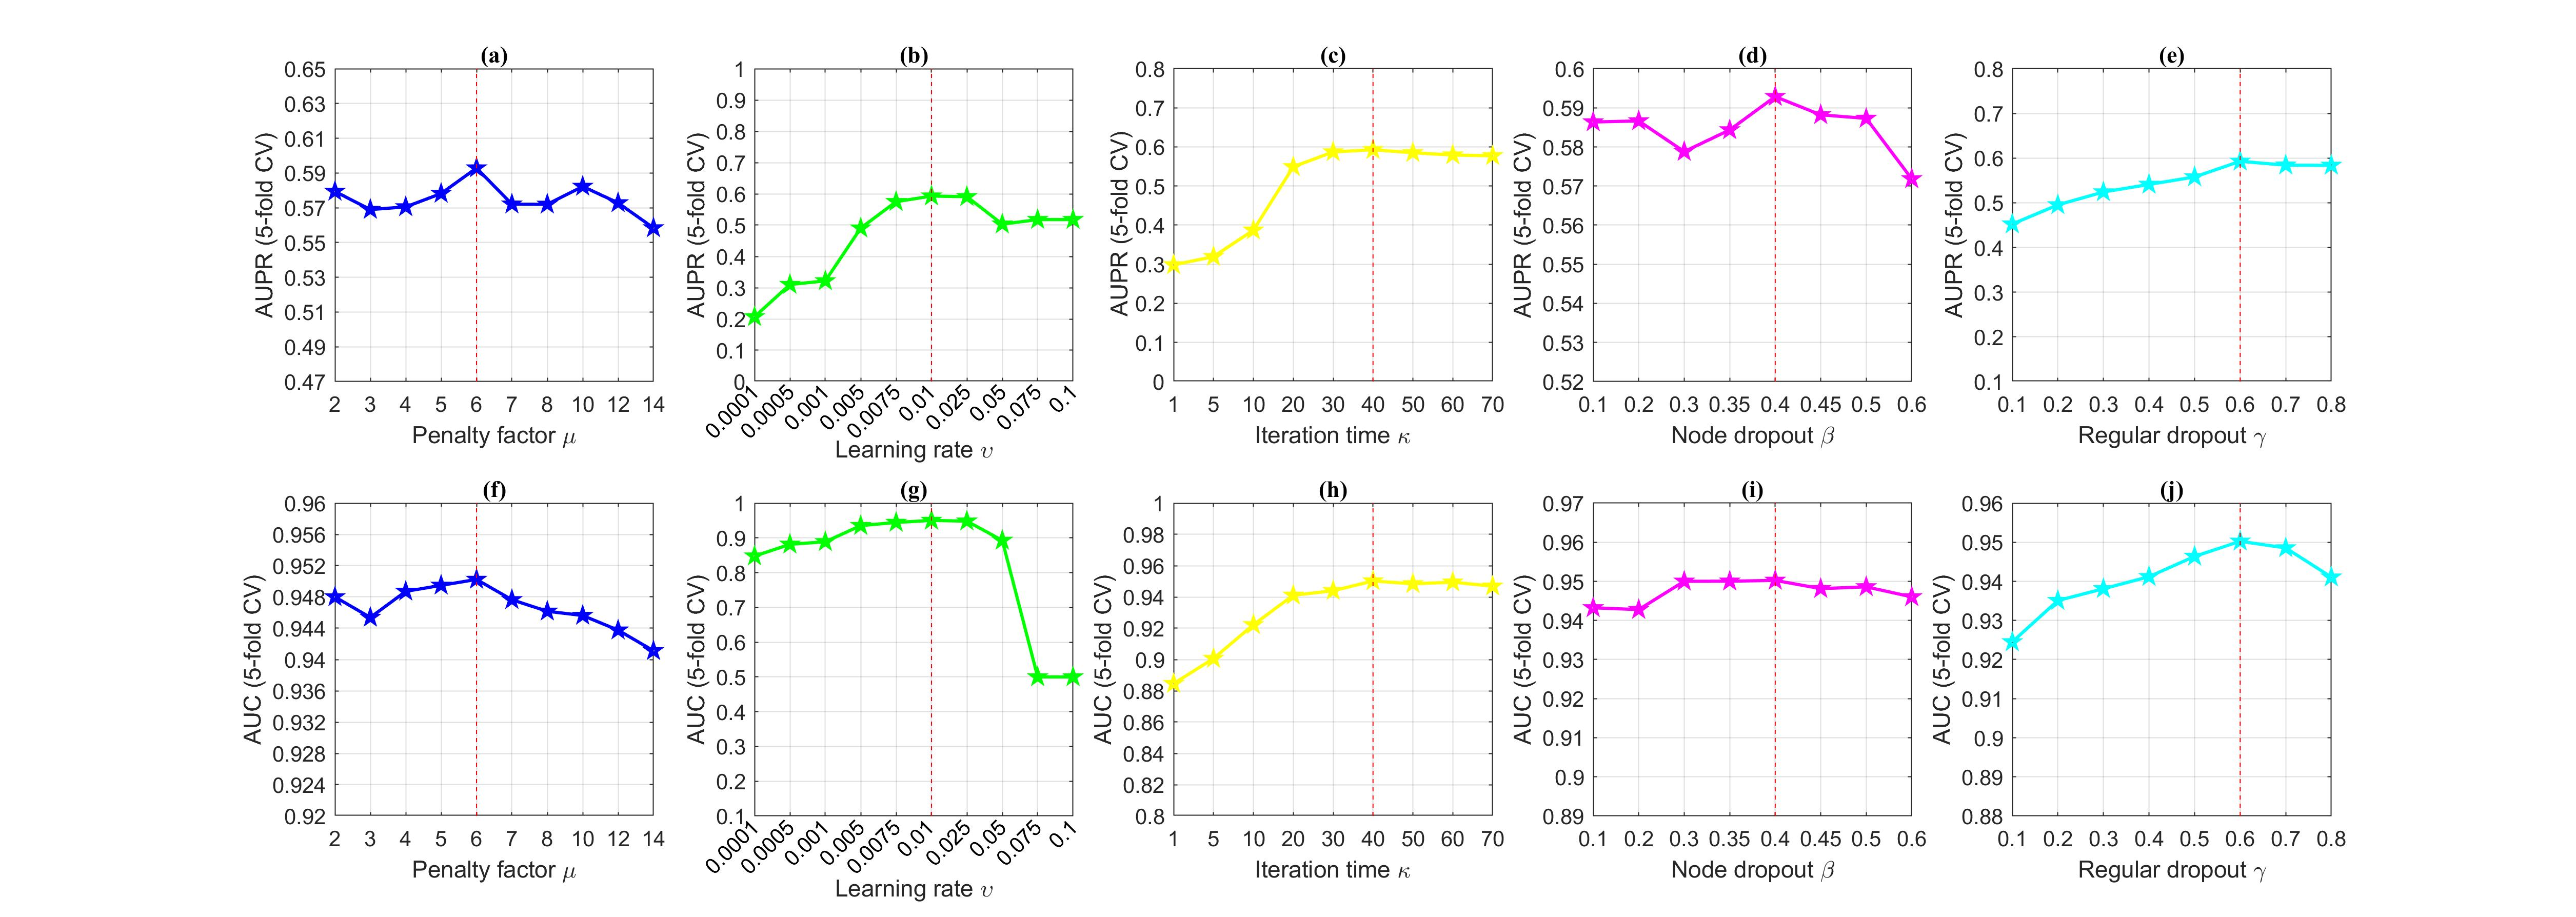
\includegraphics[width=\textwidth]{fig1.jpg}
%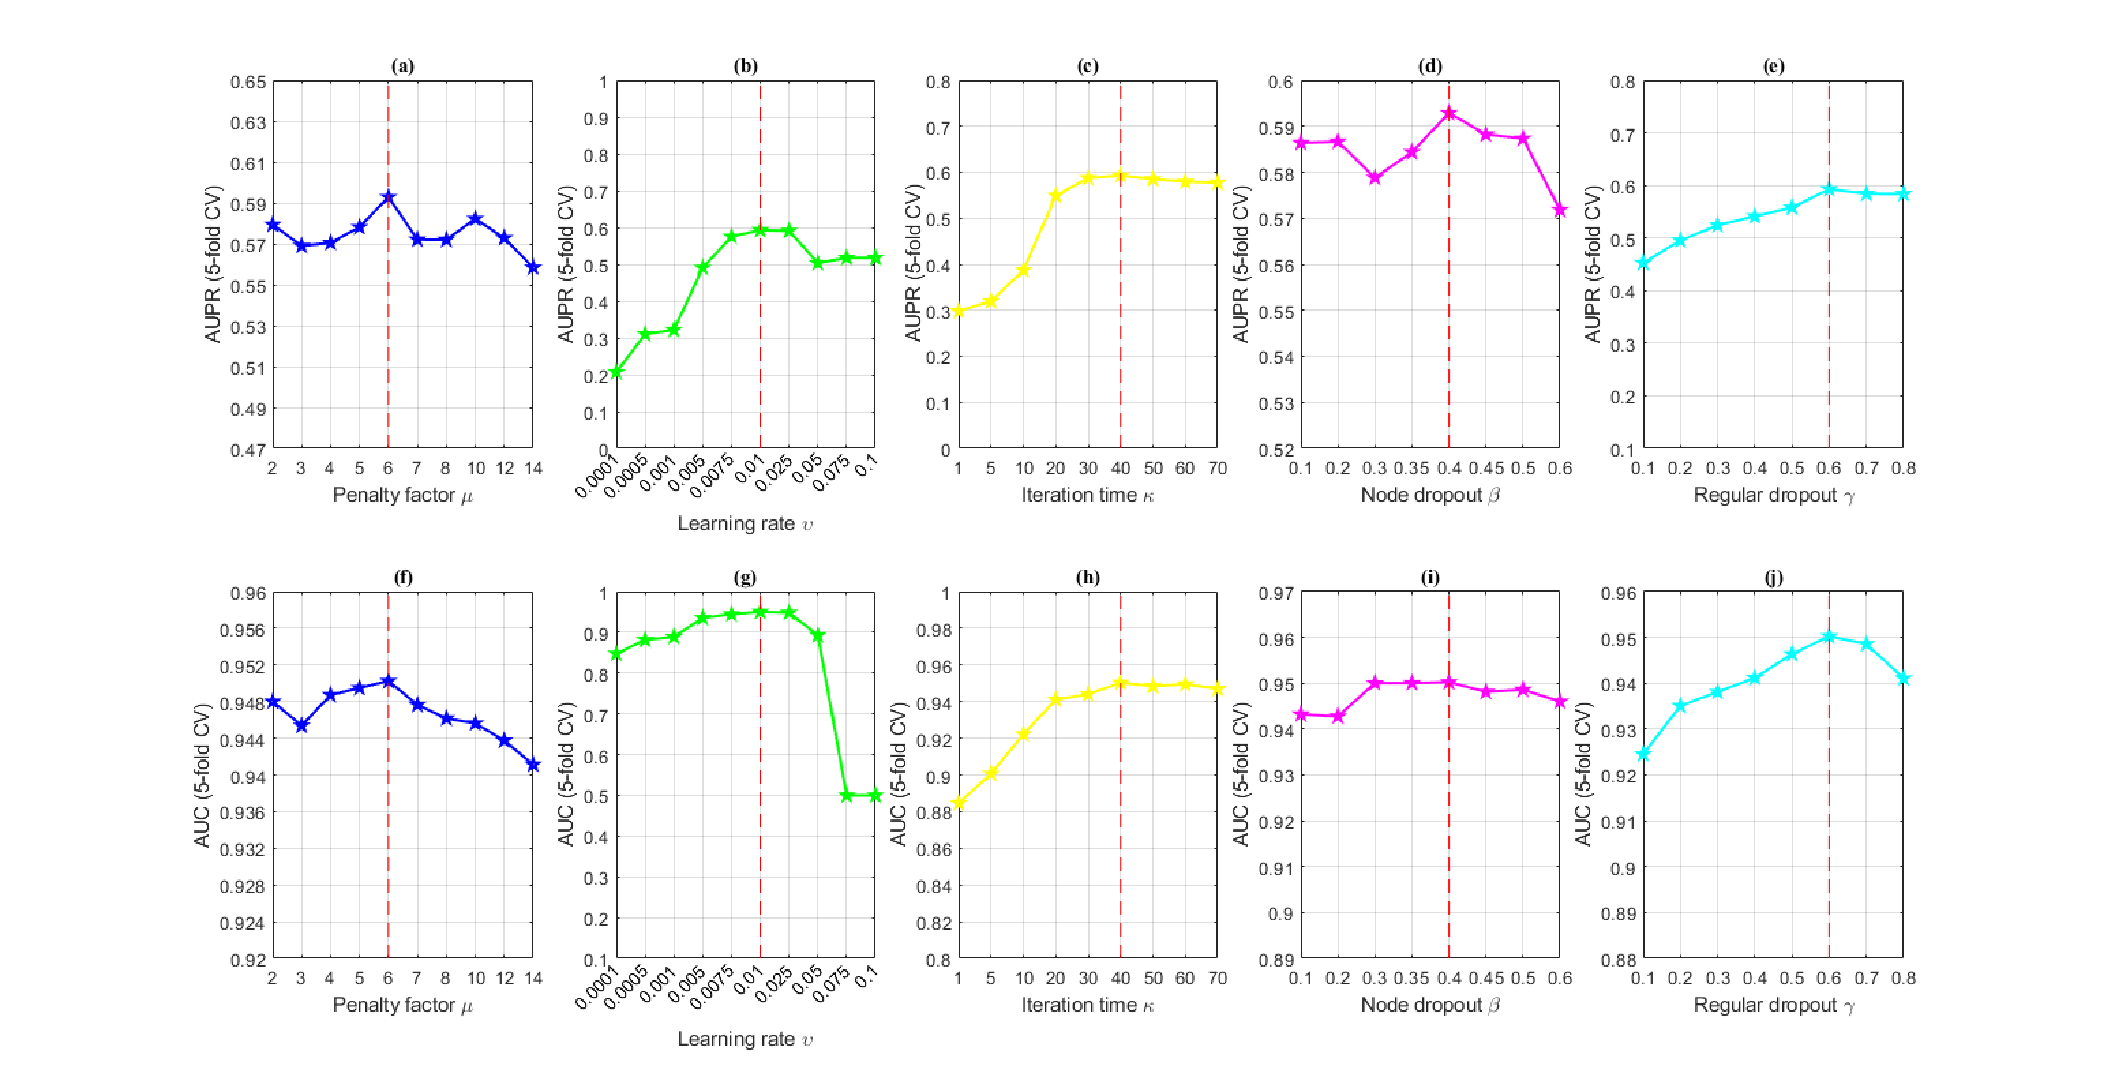
\includegraphics[height=4.5cm,width=7.5cm]{images/fig1_benckmark.pdf}
\caption{The influence of parameters of the LPI-FKLGCN model tested by 5-fold CV on the Benchmark Dataset}
\label{fig:fig2-1}
\end{figure}

%The parameter adjustment in the novel dataset are stored in the supplementary file.
%\begin{figure}[ht]
%    \centering
%\graphicspath{ {./images/} }
% 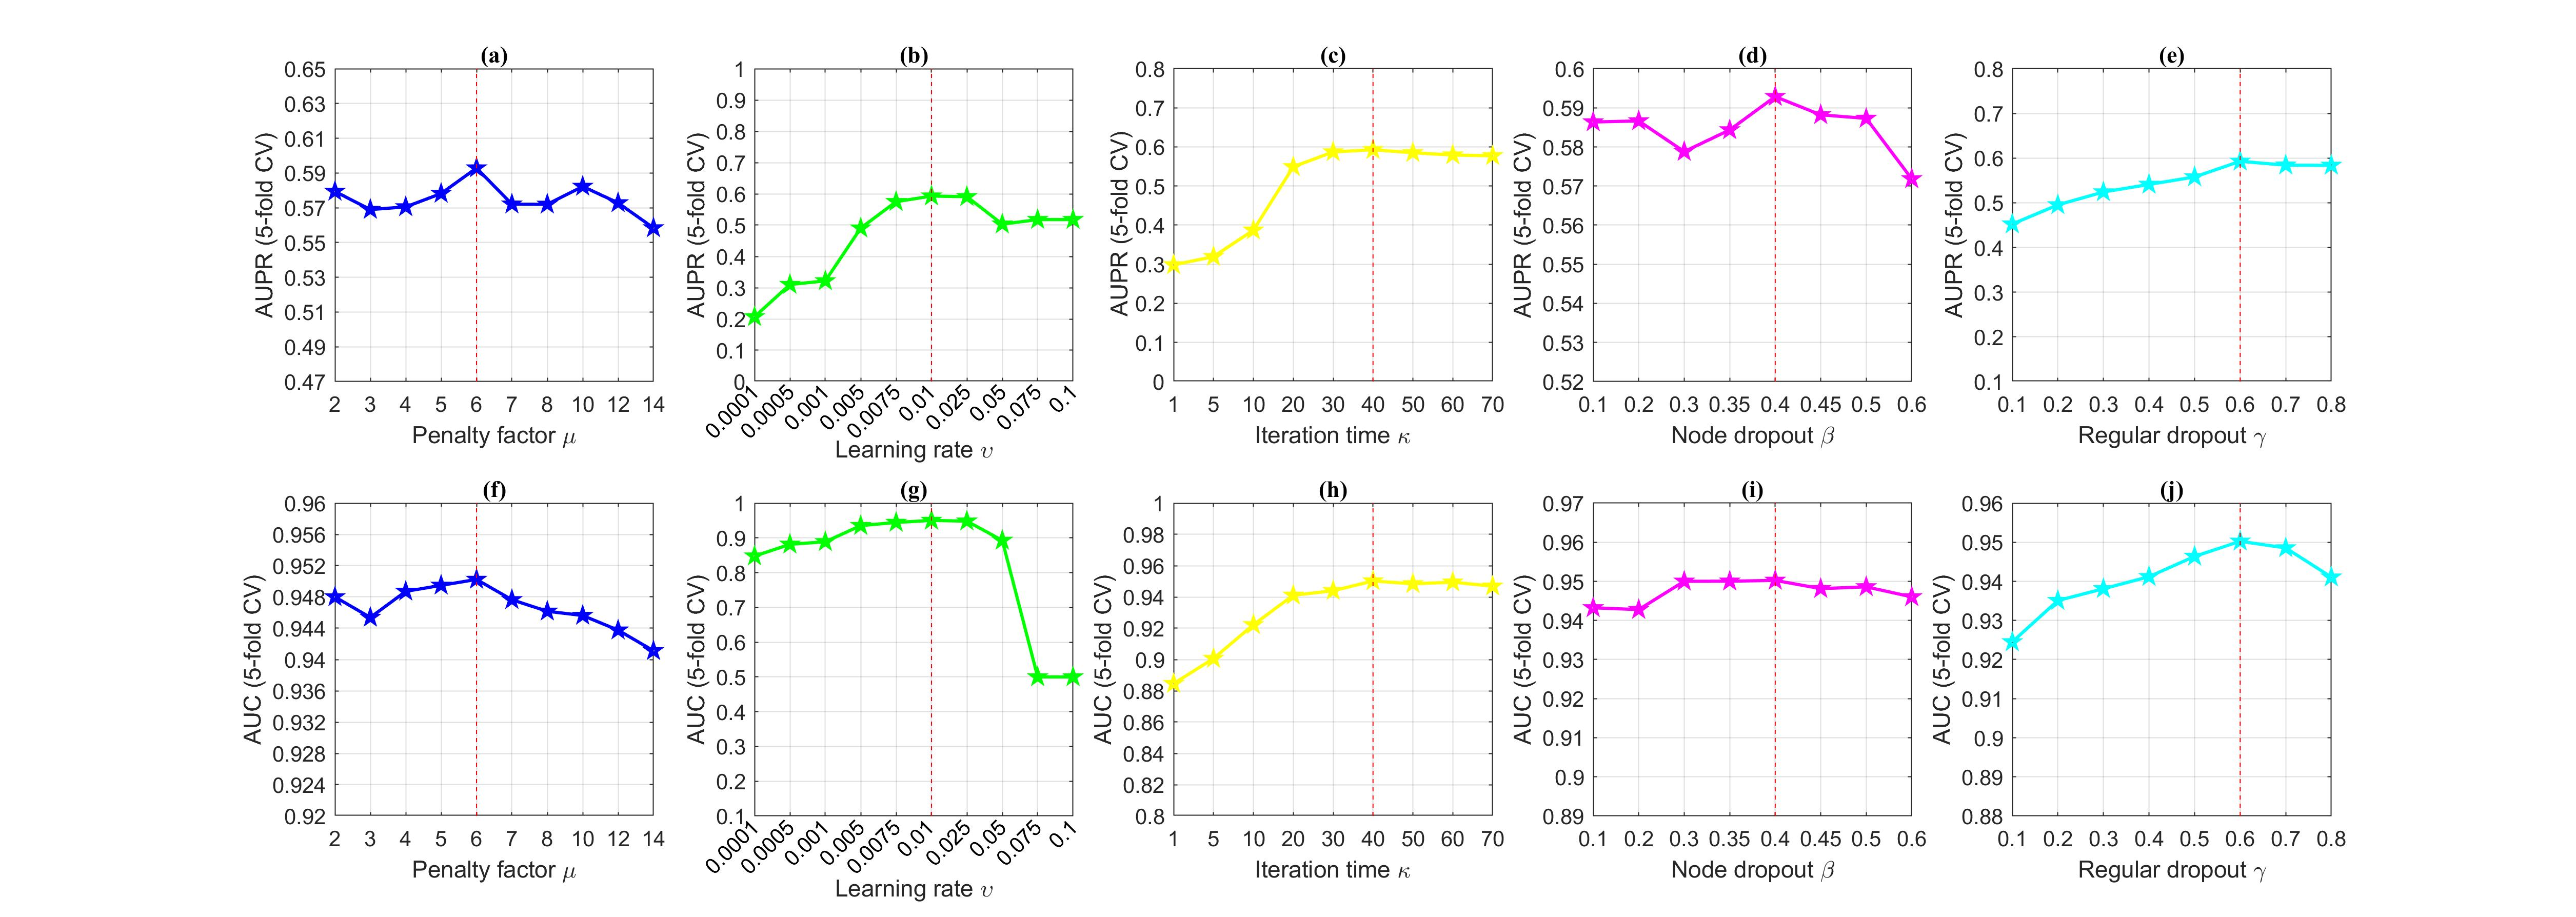
\includegraphics[width=\textwidth]{fig1.jpg}
%    \caption{Parameter adjustment in the GCN by 5-fold CV in the Novel Dataset}
%    \label{fig:fig2-2}
%\end{figure}

\subsection*{2.3 Overall performance analysis}
The impact of fast kernel learning and multi-layer graph convolution layers are shown in the Table \ref{tab:parameter1}.
\begin{itemize}
\item kernel fusion with average weights
\item kernel fusion with SNF
\item Graph conv 1 layer
\item Graph conv 2 layer
\item Graph conv 3 layer
\end{itemize}
\begin{table}[ht]
\centering
 \caption{\label{tab:parameter1}The results of comparison with FKLGCN variants. (350 words max). Example legend text.}
\begin{threeparttable}[b]
\begin{tabular}{|l|l|l|l|l|l|l|l|l|}
\hline
Dataset & Models & AUPR & AUC &	F1_score & Accuracy	& Recall & Specificity & Precision\\
\hline
\multirow{4}{5em}{Benchmark Dataset} 
& Fuse_AVG\tnote{1} & 0.2795 & 0.8736 & 0.2891 & 0.9220 & 0.4464 & 0.9395 & 0.2138\\
& Fuse_SNF\tnote{2} & 0.3434	& 0.8874 & 0.3737	& 0.9351 & 0.5451	& 0.9494 & 0.2843\\
& GCN with 1 layer conv & 0.5504 & 0.9476 & 0.5367 & 0.9628 & 0.6064 & 0.9759 & 0.4813\\ 
& GCN with 2 layer conv & 0.5655 & 0.9487 & 0.5444 & 0.9616 & 0.6050 & 0.9733 & 0.4710\\
& GCN with 3 layer conv& 0.5928 & 0.9502 & 0.5424 & 0.9705 & 0.6113 & 0.9784 & 0.6041\\
\hline
\multirow{4}{6em}{Novel Dataset} 
& Fuse_AVG\tnote{1} & 0.4946 & 0.9422 & 0.1655 & 0.9003 & 0.8451 & 0.9000 & 0.0908\\
& Fuse_SNF\tnote{2} & 0.5121 & 0.9480 & 0.1782 & 0.9114 & 0.8693 & 0.9114	& 0.0988\\
& GCN with 1 layer conv & 0.4469 & 0.9600 & 0.2282 & 0.9286 & 0.6566 & 0.9721 & 0.1313\\ 
& GCN with 2 layer conv & 0.4890 & 0.9602 & 0.2317 & 0.9328 & 0.8165 & 0.9441 & 0.1350\\
& GCN with 3 layer conv & 0.5212 & 0.9638 & 0.2362 & 0.9894 & 0.8859 & 0.9400 & 0.1362\\
\hline
\end{tabular}
\begin{tablenotes}
     \item[1] multiple kernel fusion with average weights
     \item[2] multiple kernel fusion with SNF
     \end{tablenotes}
     \end{threeparttable}
\end{table}


\subsection*{2.4 Comparison with other classic methods}
\begin{itemize}
\item RWR
\item CF
\item RA
\item HRWR
\item LPI-FKLKRR
\end{itemize}
\begin{itemize}
\item RWR
\item CF
\item RA
\item HRWR
\item LPI-FKLKRR
\end{itemize}

\begin{table}[ht]
\centering
\caption{\label{tab:Comparison1}The results of comparison with classical baseline methods. (350 words max). Example legend text.}
\begin{tabular}{|l|l|l|l|l|l|l|l|}
\hline
Dataset	& Metric & RWR	& CF & RA & HRWR & LPI_FKLKRR & LPI_GCN \\
\hline
\multirow{5}{9em}{Benchmark_Dataset} 
& AUPR & 0.283 & 0.236 & 0.230 & 0.330 & 0.551 & 0.593 \\ 
& AUC & 0.813 & 0.769 	& 0.845 & 0.857 & 0.794 & 0.950 \\
& Precision	& 0.354  & 0.303 & 0.414 & 0.290 & 0.519 & 0.604 \\
& Accuracy	& 0.954 & 0.951 & 0.958 & 0.943 & 0.870 & 0.971 \\
& F1_score & 0.360 & 0.299 & 0.387 & 0.334 & 0.508 & 0.542 \\
\hline
\multirow{5}{9em}{Novel_Dataset} 
&AUPR	&0.281	&0.262	&0.333	&0.247	&0.486	&0.521\\
&AUC	&0.928	&0.902	&0.940	&0.931	&0.880	&0.963\\
&Precision	&0.364	&0.361	&0.391	&0.286	&0.607	&0.136\\
&Accuracy	&0.986	&0.986	&0.986	&0.982	&0.956	&0.989\\
&F1_score	&0.3488	&0.322	&0.393	&0.339	&0.491	&0.236\\
\hline
\end{tabular}
\end{table}
Results of comparison with other classic methods are shown in Table \ref{tab:Comparison1}

\subsection*{2.5 Comparison with the state-of-the-art methods}

\begin{itemize}
\item LAGCN
\item AEMDA
\item LPI-GCNIMC
\end{itemize}

\begin{itemize}
\item LAGCN
\item AEMDA
\item LPI-GCNIMC
\end{itemize}

\begin{figure}[ht]
\centering
\subfigure[The ROC curve]{
\label{Fig.sub.1}
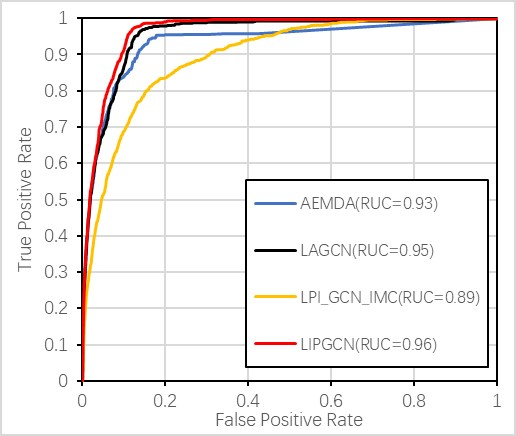
\includegraphics[width=18em]{images/fig41.jpg}}
\subfigure[The PR curve]{
\label{Fig.sub.2}
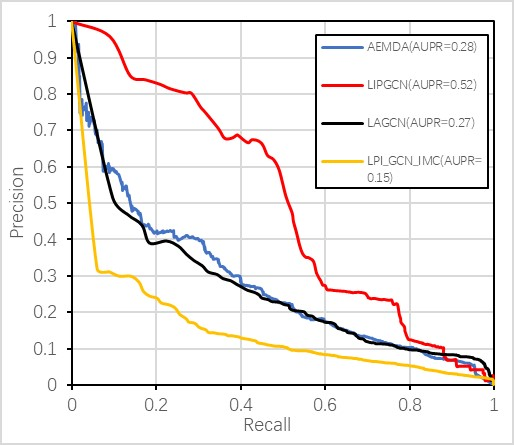
\includegraphics[width=18em]{images/fig42.jpg}}
\caption{Comparison with the excellent methods}
\label{Fig.lable3}
\end{figure}

The results of comparison with the state-of-the-art methods are shown in the Figure \ref{Fig.lable3}.

\subsection*{2.6 Case study}
TOP 10 predicted proteins for lncRNA NONHSAT145960 and TOP 10 predicted lncRNAs for protein ENSP00000401371 as shown in Table \ref{tab:caseStudy1}

In this section, we build an LAGCN model using all drug–disease associations and then predict novel associations. Because all known associations have been used to construct the prediction model, the predicted associations require verification by public literature or other available sources. Top 10 drug–disease associations predicted by LAGCN are listed in Table 6, and we can find evidence to confirm five out of them. For example, tamoxifen is capable of prolonging the lives of premenopausal women with breast cancer and decreasing the probability of recurrence, but it led to acute depression symptoms in a 34-year-old breast cancer patient [53]. Dexamethasone is a type of corticosteroid medication. It was used in the treatment of many conditions, including rheumatic problems, several skin diseases, severe allergies, asthma, chronic obstructive lung disease, croup, brain swelling, ocular pain following ophthalmic surgery and antibiotics in tuberculosis. It was also used as a direct chemotherapeutic agent in the treatment of multiple myeloma, in which dexamethasone is given in combination with lenalidomide [54].
Furthermore, we check upon the top 10 candidate diseases for carbamazepine and the top 10 candidate drugs for breast neoplasms. Table 7 shows the results of our experiments, and some of the predictions can be confirmed. For example, carbamazepine is an anticonvulsant medication used primarily in the treatment of epilepsy and neuropathic pain, but De Sarro et al. [55] have proved that carbamazepine also leads to movement disorders by potentiating the anticonvulsant activity in the DBA/2 mice animal model. Breast cancer is the leading type of cancer in women, accounting for 25 $\%$ of all cases according to Wikipedia, and countless researchers have been devoting themselves to finding treatment of it. According to Tsai et al. [56], tamoxifen and fulvestrant are widely used therapeutic agents and are considered to alter estrogen receptor (ER) signaling in ER-positive breast cancers.

\begin{table}[ht]
\centering
\caption{\label{tab:caseStudy1} The results of case study for LPIs and novel lncRNA prediction. (350 words max). Example legend text.}
\begin{tabular}{|l|l|l|l|l|l|l|l|l|}
\hline
\multirow{2}{*}{TOP 10 Rank} & \multicolumn{2}{|l|}{Protein ID: ENSP00000401371} & \multicolumn{2}{|l|}{LncRNA ID: NONHSAT145960}& \multicolumn{2}{|l|}{LncRNA ID: NONHSAT022115}\\
\cline{2-7}
 & Predicted lncRNAs & Confirm? & Predicted proteins & Confirm? & Predicted proteins & Confirm? \\
\hline
1 & NONHSAT104639  & C & ENSP00000240185 & C & ENSP00000362306 & C
\\
2 & NONHSAT107804 & C & ENSP00000349428	& C & ENSP00000362287 & 	C
\\
3 & NONHSAT043887  & C & ENSP00000401371	& C & ENSP00000362300 & 	C
\\
4 & NONHSAT131038  & C & ENSP00000371634	& no & ENSP00000220592  & C
\\
5 & NONHSAT072962  & no & ENSP00000258729 & C & ENSP00000385269  & C
\\
6 & NONHSAT060501  & C & ENSP00000290341	& C & ENSP00000254108  & C
\\
7 & NONHSAT054716 & C & ENSP00000379144 & C & ENSP00000381031 & C
\\
8 & NONHSAT022112 & no & ENSP00000338371 & C & ENSP00000258729 & C
\\
9 & NONHSAT092691 & C & ENSP00000354951	& no & ENSP00000371634 & no
\\
10 & NONHSAT103491 & no & ENSP00000309558 & no & ENSP00000290341  & C
\\
\hline
\end{tabular}
\end{table}

%出现某些预测的蛋白质的与lncRNA的值近似为0,可能原因其一,本身蛋白质与lncRNAs的关联数只有1,2不超过10个。
TOP 10 predicted proteins for novel lncRNA are shown in Table \ref{tab:caseStudy1}

TOP 10 predicted proteins for novel lncRNA are shown in Table \ref{tab:caseStudy1}

TOP 10 predicted proteins for novel lncRNA are shown in Table \ref{tab:caseStudy1}

TOP 10 predicted proteins for novel lncRNA are shown in Table \ref{tab:caseStudy1}

TOP 10 predicted proteins for novel lncRNA are shown in Table \ref{tab:caseStudy1}

TOP 10 predicted proteins for novel lncRNA are shown in Table \ref{tab:caseStudy1}

\section*{Discussion}
%The Discussion should be succinct and must not contain subheadings.
%1.	简明扼要重申论文的主题及其重要性。
%2.	简要重述你完成了哪些内容的研究。
%3.	概括你的主要发现及其重要性。
%4.	指出你得到的结果的意义,例如奠定了什么,丰富了什么,纠正了什么,补充了什么,提出了什么。
%5.	解释论文工作从多大程度上接近了引言中所指出的需求。
%6.	论文工作的不足。例如受目前研究条件所限,未能获取某些更高的条件才能处理的问题,概述未来可以开展什么研究。
First of all, LPI-FKLGCN model obtains rich information about lncRNAs and proteins from different data sources, which are represented as a variety of features and similarities.They are then fused by fast kernel learning to generate a comprehensive lncRNA similarity and a comprehensive protein similarity. Then, a set of lncRNAs and a set of protein embedded representation vectors are generated through the nonlinear multi-layer graph convolutional network combined with the comprehensive similarity and interaction matrix of lncRNAs and proteins. Finally, the interaction probability fraction matrix is obtained by decoding.

First of all, LPI-FKLGCN model obtains rich information about lncRNAs and proteins from different data sources, which are represented as a variety of features and similarities.They are then fused by fast kernel learning to generate a comprehensive lncRNA similarity and a comprehensive protein similarity. Then, a set of lncRNAs and a set of protein embedded representation vectors are generated through the nonlinear multi-layer graph convolutional network combined with the comprehensive similarity and interaction matrix of lncRNAs and proteins. Finally, the interaction probability fraction matrix is obtained by decoding.

\section*{Methods}
In this section, we first construct a heterogeneous network integrating the lncRNA comprehensive similarity network, the protein comprehensive similarity network and known lncRNA-protein interaction network. Then, we generate multiple kernels for lncRNAs and proteins, and fuse these base kernels into a lncRNA comprehensive similarity and a protein comprehensive similarity, respectively. Thirdly, we deploy the multi-layer graph convolution network on the constructed heterogeneous network so as to generate the embedding representation vectors for lncRNAs and proteins. The combination of multi-layer embedding can integrate proximity of different order to improve the next prediction. Finally, the predicted lncRNA-protein interaction probability matrix is obtained by decoding. 

\subsection*{Construction of a heterogeneous lncRNA-protein network}
In order to make more accurate prediction, the LPI-FKLGCN model makes full use of multi-source information, such as known lncRNA-protein interaction, lncRNA and protein sequence, lncRNA expression profile and protein GO to generate multiple similarity kernels and feature kernels. The base kernels will be combined to a comprehensive similarity matrix by the fast kernel fusion. The heterogeneous lncRNA-protein network is constructed by a lncRNA-protein interaction network, a lncRNA comprehensive similarity network and a protein comprehensive similarity network. Assume that matrix ${{I}} \in {\Re ^{m \times n}}$ represents the adjacency matrix for lncRNA-protein interaction network. If there is an interaction between lncRNA ${{l_i}}$ and protein ${{p_j}}$, ${{I}}(i,j)$ assigns 1, otherwise it assigns 0. $1 \le i \le m$, $1 \le j \le n$, $m$, $n$ are the number of lncRNAs and proteins in the interaction profile. The adjacency matrix of the comprehensive similarity networks are respectively denoted as ${{{K}}_l}$ and ${{{K}}_p}$. At last, the adjacency matrix of the heterogeneous network ${A^ \sim }$ can be defined as equation (\ref{eq:adjmatrix}):
\begin{equation}\label{eq:adjmatrix}
{A^ \sim } = \left[ {\begin{array}{*{20}{c}}
{{{{K}}_l}}&{{I}}\\
{{{{I}}^T}}&{{{{K}}_p}}
\end{array}} \right] \in {\Re ^{(m + n) \times (m + n)}}
\end{equation}
\subsection*{Generate multiple kernels for lncRNAs and proteins}
\subsubsection*{Sequence feature kernels for lncRNAs and proteins}
We extracted the sequence features of lncRNAs and proteins by the same way as in the previous literature \cite{Shen2019}. The lncRNA sequences are expressed by Conjoint Triad, and the protein sequences are expressed by Pseudo Position-Specific Score Matrix. Then, the Sequence Feature kernels ${{K}}_l^{SF}$ and ${{K}}_p^{SF}$ can be extracted by the Radial Basis Function (RBF) kernel.

\subsubsection*{Sequence similarity kernels for lncRNAs and proteins}
The lncRNA Sequence Similarity (SS) kernels ${{K}}_l^{SS}$ can be calculated by normalized Smith-Watermark (SW) score as\cite{Shen2019}
\begin{equation}
{{K}}_l^{SS}({l_i},{l_j}) = \frac{{SW({S_{{l_i}}},{S_{{l_j}}})}}{{\sqrt {SW({S_{{l_i}}},{S_{{l_j}}})SW({S_{{l_i}}},{S_{{l_j}}})} }} \label{eq:SSim}
\end{equation}
where ${{S_{{l_i}}}}$ denotes the sequence of lncRNA ${l_i}$, $SW( \cdot )$ represents the Smith-Watermark score. Similarly, if we put protein sequences ${{S_{{p_i}}}}$ into equation (\ref{eq:SSim}), we can also extract the protein Sequence Similarity kernels ${{K}}_p^{SS}$.

\subsubsection*{Gaussian interaction profile kernels for lncRNAs and proteins}
The Gaussian Interaction Profile (GIP) kernel actually is a measurement of network topology similarity\cite{VanLaarhoven2011}, which can be calculated through the lncRNA-protein interaction profile. lncRNA GIP kernel ${{K}}_l^{GIP}$ is calculated as equation (\ref{eq:GIP_sim}):
\begin{equation} \label{eq:GIP_sim}
{{K}}_l^{GIP}({l_i},{l_j}) = \exp ( - {\gamma _l}{\left\| {{IP}({l_i}) - {IP}({l_j})} \right\|^2})
\end{equation}
where vector ${{{IP}}({l_i})}$ represents the interaction profile for lncRNA $l_i$, which actually is the ith row vector of the interaction matrix ${{I}}$. It represents whether there is a interacting protein with the lncRNA $l_i$. Similarly, vector ${{{IP}}({p_i})}$ is the ith column vector of the matrix ${{I}}$. The GIP kernel for proteins ${{K}}_p^{GIP}$ can also be calculated by substituting ${{{IP}}({p_i})}$ into the equation(\ref{eq:GIP_sim}).
   ${\gamma _l}$ and ${\gamma _p}$ are parameter bandwidths, which can be calculated as: ${\gamma _l} = {{{{\gamma '}_l}} \mathord{\left/
 {\vphantom {{{{\gamma '}_l}} {(\frac{1}{m}\sum\limits_{i = 1}^m {{{\left\| {{{IP}}({l_i})} \right\|}^2}} )}}} \right.
 \kern-\nulldelimiterspace} {(\frac{1}{m}\sum\limits_{i = 1}^m {{{\left\| {{IP}({l_i})} \right\|}^2}} )}}$, where ${\gamma '}$ are usually set to 1.

\subsubsection*{Expression kernel for lncRNAs}
The lncRNA Expression profiles are obtained from the database NONCODE, each of which is represented as a 24-dimension vector, corresponding to 24 cell types. At last, the lncRNA Expression kernel ${{K}}_l^{Exp}$ can also be extracted by the Radial Basis Function as in the literature\cite{Buhmann2004}.

\subsubsection*{GO kernel for proteins}
Gene ontology (GO) describes biomolecules or gene products in terms of biological processes, molecular functions and cellular components. GO has become a commonly used protein feature in interaction prediction models. We downloaded GO terms from the database GOA\cite{Wan2013} to measure GO similarity between two proteins. Jaccard similarity, namely the overlap ratio of GO terms related to two proteins, is used to computed GO kernels of two proteins ${{K}}_p^{GO}$ as equation (\ref{eq:GO_kernel}).
\begin{equation}\label{eq:GO_kernel}
{{K}}_p^{GO}({p_i},{p_j}) = \frac{{\left| {G{O_{{p_i}}} \cap G{O_{{p_j}}}} \right|}}{{\left| {G{O_{{p_i}}} \cup G{O_{{p_j}}}} \right|}}
\end{equation}
where ${G{O_{{p_i}}}}$ is the GO terms related with protein ${p_i}$, $ \cap $ is the intersection of two sets, $ \cup $ is the union of two sets.

Above all, four base kernels for lncRNAs ${{K}}_l^{SF}$, ${{K}}_l^{SS}$, ${{K}}_l^{GIP}$, ${{K}}_l^{Exp}$ are generated, and four base kernels for proteins ${{K}}_p^{SF}$, ${{K}}_p^{SS}$, ${{K}}_p^{GIP}$, ${{K}}_p^{GO}$ are generated.

\subsection*{Comprehensive similarity network by fast kernel learning}
A variety of similarity and features can depict biological entities from different perspectives, so as to make better interaction prediction. In this paper, a linear combination strategy is used to quickly fuse multiple similarities and features\cite{He2008,Shen2019}. A comprehensive  similarity ${{{K}}_l}$ can be combined as: ${{{K}}_l} = \sum\limits_{i = 1}^4 {w_l^i} {{K}}_l^i,\;\;\;{{K}}_l^i \in {\Re ^{m \times m}}$, where ${w_l^i}$ are combination weights, $\sum\limits_{i = 1}^4 {{w_i}}=1$, and ${{K}}_l^i$ are base kernels for lncRNAs. Similarly, the protein comprehensive similarity ${{{K}}_p}$ also can be calculated by substituting the base kernels of proteins ${{K}}_p^i \in {\Re ^{n \times n}}$ and combination weights ${w_p^i}$ into the combination equation like lncRNAs. 

In the ideal state, the comprehensive similarity of fusion should satisfy ${{{K}}^{ideal}} = {{I}}\times{{{I}}^T}$. As long as the appropriate weight ${w}$ can be determined and the following formula $\min \left\| {{{K}} - {{K}^{ideal}}} \right\|_F^2$ can be satisfied, the goal of multi-kernel fusion can be achieved. In order to avoid over-fitting, a regularization term $\lambda {\left\| {w} \right\|^2}$ is added in the fusion process, and the objective function can be transformed into the equation (\ref{eq:fusionObjection}):
\begin{equation}\label{eq:fusionObjection}
\begin{array}{l}
\mathop {\min }\limits_{{{w,K}}} \;\left\| {{{K}} - {{{K}}^{ideal}}} \right\|_F^2 + \lambda {\left\| {w} \right\|^2}\\
\;s.t.\;\;\sum\limits_{i = 1}^4 {{w_i}}  = 1
\end{array}
\end{equation}
where ${\left\|  \cdot  \right\|_F}$ represents Frobenius norm, ${{K}}$ represents ${{{K}}_l}$ or ${{{K}}_p}$,${{{K}}_l^i}$ or ${{{K}}_p^i}$ are base kernels of lncRNAs or proteins. {w} represents ${{w}_l}$ or ${{w}_p}$, $w_l^i$ or $w_p^i$ are combination weights. The tradeoff parameter $\lambda$ is initialed to 2000 in this study. We call the Matlab tool function CVX to optimize the combination weights {{w}} and get the comprehensive similarity {K} for lncRNAs and proteins, respectively.  

\subsection*{Encoding by multi-layer graph convolution network}
The graph convolutional network (GCN) which extends Convolutional Neural Networks into graph architecture has been applied in the field of biological information processing and achieved excellent performance. For example, %GCN has been used in the polypharmacy side effects prediction\cite{Zitnik2018},
microbe-drug association prediction\cite{Long2020d}, computational drug discovery\cite{Sun2020b} and drug-disease association prediction\cite{Yu2020d}.
We intend to construct a encoder by GCN and launch the GCN on the heterogeneous network ${A^ \sim }$ to learn the low-dimensional representations of lncRNAs and proteins. The graph $G$ to be input into the GCN is defined as:
\begin{equation}\label{eq:inputG}
G = \left[ {\begin{array}{*{20}{c}}
{\mu  \sim {K_l}}&I\\
{{I^T}}&{\mu  \sim {K_p}}
\end{array}} \right]
\end{equation}
where $\mu$ is a penalty factor indicating the importance of similarity in the process of information propagation. 
The GCN encoder for processing this lncRNA-protein heterogeneous graph is defined as follows:
\begin{equation}\label{eq:encoder}
{V^{(l + 1)}} = f({V^{(l)}},G) = \sigma ({D_G^{ - \frac{1}{2}}}G{D_G^{ - \frac{1}{2}}}{V^{(l)}}{W^{(l)}})
\end{equation}
where $\sigma ( \cdot )$ is an non-linear activation function, ${V^{(h)}}$ is the output embedding representation vector of the h-layer, $W^{(h)}$ is the training weight matrix of h-layer, ${D_G} = diag(\sum\nolimits_j {{G_{ij}}} )$ is the degree matrix of graph $G$. In order to accelerate the learning process and improve the generalization performance, the exponential linear units (ELUs) are adopted as the non-linear activation function $\sigma ( \cdot )$ for all the GCN layers \cite{Clevert2016}. The initialization of the embedding presentation vector is defined as: ${V^{(0)}} = \left[ {\begin{array}{*{20}{c}} 0&I\\ {{I^T}}&0 \end{array}} \right]$. So, the h-layer of the GCN encoder can be initialized as: ${V^{(h)}} = \sigma ({D_G^{ - \frac{1}{2}}}G{D_G^{ - \frac{1}{2}}}{V^{(0)}}{W^{(0)}})$, where ${V^{(h)}} \in {\Re ^{(m + n) \times k}}$ is the h-layer embedding representation vectors of the graph $G$, parameter $k$ is the embedded dimension, and ${W^{(0)}} \in {\Re ^{(m + n) \times k}}$ is an weight matrix. For all the layers ($h=1,2,...,H$ layers) of the GCN, the propagation progress follow the equation (\ref{eq:encoder}). Each time the graph passes through one GCN layer, one set of k-dimensional embedding vectors are generated. The embedding representation vectors of different GCN layers capture different order proximity of neighbors in heterogeneous networks. To advoid over-fitting, our model adopt regular dropout $\gamma $  and node dropout $\beta $ to the GCN. The node dropout can be thought of as the training of different models on different small networks which can be integrated to predict unknown LPIs. Therefore, the GCN encoder can be converted to:
\begin{equation}
{V^{(h)}} = \sigma ({D_G^{ - \frac{1}{2}}}[(1-\beta)G]{D_G^{ - \frac{1}{2}}}[(1-\gamma){V^{(0)}}]{W^{(0)}})
\end{equation}

Finally, the final embedding vectors of lncRNAs ${V_L} \in {\Re ^{m \times k}}$ and the final embedding vectors of proteins ${V_P} \in {\Re ^{n \times k}}$ are generated by the following equation: 
\begin{equation}
\left[ {\begin{array}{*{20}{c}} {{V_L}}\\ {{V_P}} \end{array}} \right] = \sum {{a_h}{V^h}}
\end{equation}
where ${a_h}$ is initialized as $1/(h + 1),{\kern 1pt} {\kern 1pt} h = 1,2,...,H$ and can be learned automatically through the GCN. 

\subsection*{Decoding and prediction}
At last, to predict the unknown LPIs, a bi-linear activation function sigmoid is used as a decoder:
\begin{equation} \label{eq:decoder}
I' = sigmoid({V_L}W'V_P^T)
\end{equation}
where $W' \in {\Re ^{k \times k}}$ is a training weight matrix. $I'$ is the predicted score matrix whose member $I'(i,j)$ indicates the probability that lncRNA $l_i$ will interact with $p_j$. The training weight ${W^{(h)}}$ and $W'$ matrix can be initialized by the Xaiver method\cite{Glorot2010UnderstandingNetworks}.

The benchmark dataset is unbalanced, because the number of known interactions is far less than the total number of lncRNA-protein pairs. So, we optimize our FKLGCN model by minimizing the loss function:
\begin{equation} \label{eq:LOSSr}
Loss =  - \frac{1}{{m \times n}}(\lambda  \times \sum\nolimits_{(i,j) \in \Delta } {\log I'(i,j)}  + \sum\nolimits_{(i,j) \in \nabla } {\log (1 - I'(i,j)} ))
\end{equation}
where $\Delta $ denotes the set of known interacted lncRNA-protein pairs (positive samples), and $\nabla $ denotes the set of all the other lncRNA-protein pairs (negative samples). $\lambda  = \left| \nabla  \right|/\left| \Delta  \right|$, where $\left| \nabla  \right|$. Inspired by the study\cite{Yu2020c}, the Adam optimizer is adopted to minimize the loss function\cite{Kingma2015Adam:Optimization}.

\bibliography{mendeley}
\section*{Acknowledgements (not compulsory)}
This work was supported by the National Nature Science Foundation of China (Grant Nos. 61702054 and 62072169), the National Key Research and Development Program (Grant Nos. 2017YFC1311003), and the Training Program for Excellent Young Innovators of Changsha (Grant No. kq2009093).
\section*{Author contributions statement}
W.L., S.W. and H.G. conceptualized the work and planned the procedure of experiments; H.G. collected the data; W.L. implemented all the experiments, analysed the results, and drafted the manuscript. All the authors have read and supported the final edition. 
\section*{Additional information}
To include, in this order: 
\textbf{Access code} (where applicable); 
All the datasets collected in this study and codes available are included in GitHub: https://github.com/vivian457/LPI-FKLGCN.

\textbf{Competing interests: All authors declare no competing interests.} (mandatory statement). 

The corresponding author is responsible for submitting a \href{http://www.nature.com/srep/policies/index.html#competing}{competing interests statement} on behalf of all authors of the paper. This statement must be included in the submitted article file.
\end{document}
